\section{Hardware beskrivelse}

% BDD  L.A.M.P.
\subsection{BDD L.A.M.P.}
\begin{figure}[H] \centering
    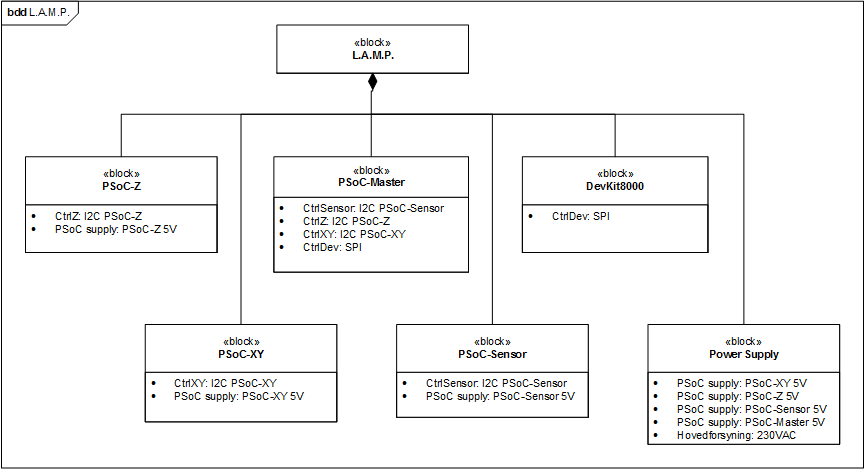
\includegraphics[width=\textwidth]{0_Filer/Figuer/5_HW_Design/bddLAMPvers3.png}
    \caption{BDD L.A.M.P.}
    \label{fig:bddLAMP}
\end{figure}
I figur \ref{fig:bddLAMP} er blok definitions diagrammet over det overordnede L.A.M.P system, diagrammet indeholder signal navne og forbindelserne mellem blokkene.

% BDD  XY-Control
\subsection{BDD XY-Control}
\begin{figure}[H] \centering
    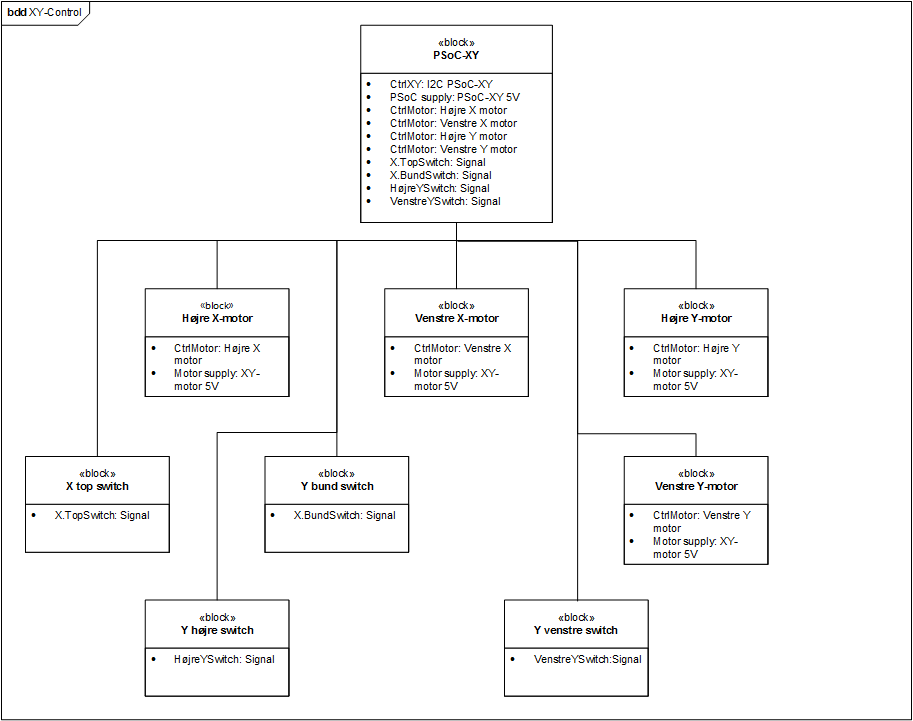
\includegraphics[width=\textwidth]{0_Filer/Figuer/5_HW_Design/bddPSoC1vers2.png}
    \caption{BDD XY-Control}
    \label{fig:bddXY}
\end{figure}
I figur \ref{fig:bddXY} er blok definitions diagrammet for XY-Control, den består af en PSoC der styre X og Y motorerne, diagrammet indeholder signal navne og forbindelserne mellem blokkene.

% BDD  Z-Control
\subsection{BDD Z-Control}
\begin{figure}[H] \centering
    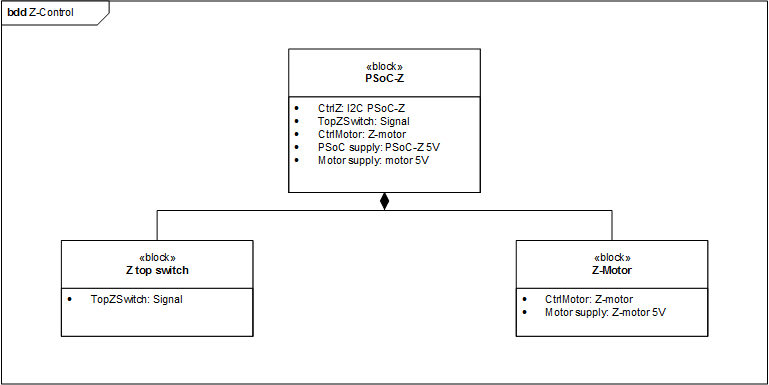
\includegraphics[width=\textwidth]{0_Filer/Figuer/5_HW_Design/bddPSoC2vers2.png}
    \caption{BDD Z-Control}
    \label{fig:bddZ}
\end{figure}
I figur \ref{fig:bddZ} er blok definitions diagrammet for Z-Control, den består af en PSoC der styre Z motoren og selve lampen, diagrammet indeholder signal navne og forbindelserne mellem blokkene.

% BDD Sensor-Control
\subsection{BDD Sensor-Control}
\begin{figure}[H] \centering
    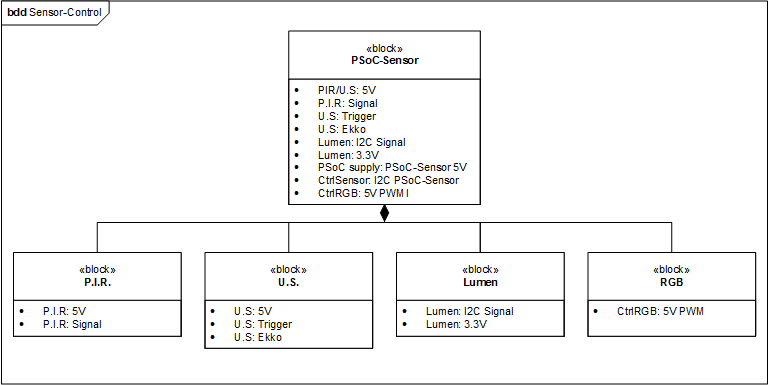
\includegraphics[width=\textwidth]{0_Filer/Figuer/5_HW_Design/bddPSoC3vers2.png}
    \caption{BDD Sensor-Control}
    \label{fig:bddSensor}
\end{figure}
I figur \ref{fig:bddSensor} er blok definitions diagrammet for Sensor-Control, den består af en PSoC der modtager information fra sensorerne, diagrammet indeholder signal navne og forbindelserne mellem blokkene.

% IBD L.A.M.P.
\subsection{IBD L.A.M.P.}
\begin{figure}[H] \centering
    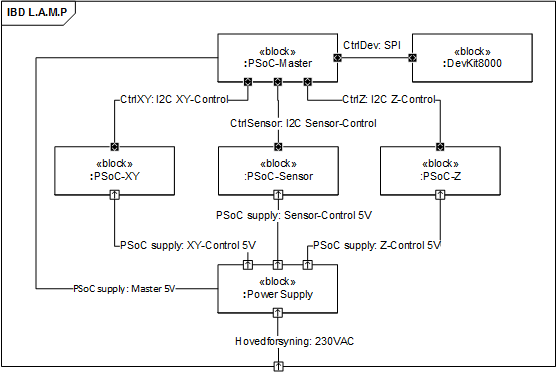
\includegraphics[width=\textwidth]{0_Filer/Figuer/5_HW_Design/IBD_LAMP_vers3.png}
    \caption{IBD L.A.M.P.}
    \label{fig:ibdLAMP}
\end{figure}
I figur \ref{fig:ibdLAMP} er det interne blok diagram over hele systemet L.A.M.P, diagrammet indeholder signal navne og forbindelserne mellem blokkene.

% IBD XY-Control
\subsection{IBD XY-Control}
\begin{figure}[H] \centering
    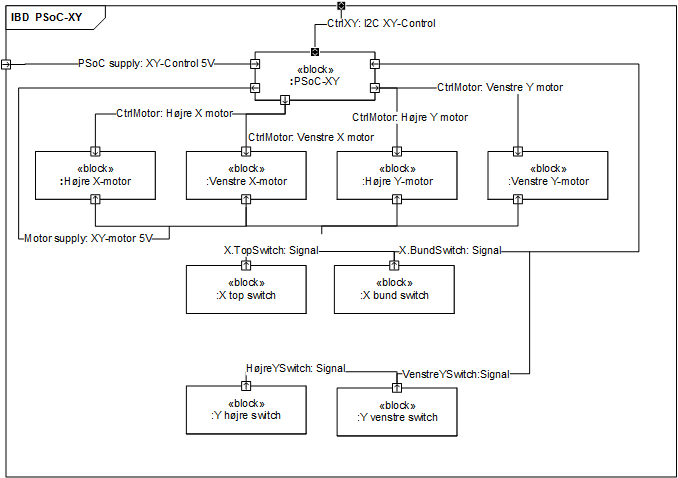
\includegraphics[width=\textwidth]{0_Filer/Figuer/5_HW_Design/IBD_PSoC1_vers3.png}
    \caption{IBD XY-Control}
    \label{fig:ibdXY}
\end{figure}
I figur \ref{fig:ibdXY} er det interne blok diagram for PSoC1, denne PSoC styre X og Y motorerne, diagrammet indeholder signal navne og forbindelserne mellem blokkene.

% IBD Z-Control
\subsection{IBD Z-Control}
\begin{figure}[H] \centering
    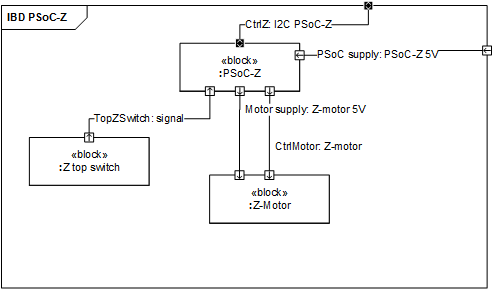
\includegraphics[width=\textwidth]{0_Filer/Figuer/5_HW_Design/IBD_PSoC2_vers3.png}
    \caption{IBD Z-Control}
    \label{fig:ibdZ}
\end{figure}
I figur \ref{fig:ibdZ} er det interne blok diagram for PSoC2, denne PSoC styre Z motoren og selve lampen, diagrammet indeholder signal navne og forbindelserne mellem blokkene.

% IBD Sensor-Control
\subsection{IBD Sensor-Control}
\begin{figure}[H] \centering
    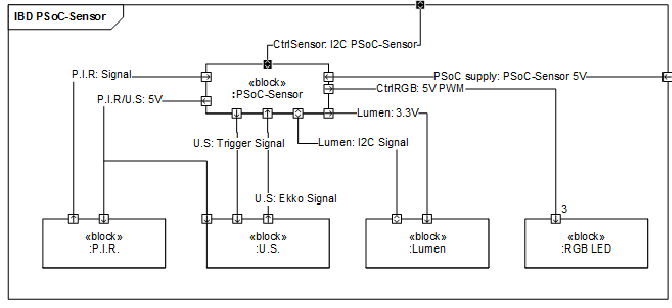
\includegraphics[width=\textwidth]{0_Filer/Figuer/5_HW_Design/IBD_PSoC3_vers3.png}
    \caption{IBD Sensor-Control}
    \label{fig:ibdSensor}
\end{figure}
I figur \ref{fig:ibdSensor} er det interne blok diagram for PSoC3, denne PSoC modtager information fra sensorerne, diagrammet indeholder signal navne og forbindelserne mellem blokkene.

% Grænseflade
\subsection{Grænseflade}

% PSoC-Master
\subsubsection{PSoC-Master}
1 PSoC, 1 stk. Nokia 5110 display.
\begin{itemize}
    \item PSoC-Master står for kommunikationen mellem Devkit8000 og XY-, Z- og Sensor PSoCs.
    \item Nokia 5110 diplay brugt til debugging til at kontrollere kommunikationen mellem Devkit8000 og PSoC-Master.
     PSoC-manual\footnote{\url{http://www.cypress.com/file/46056/download}}
\end{itemize}

% XY-Control
\subsubsection{PSoC-XY}
1 PSoC, 2 stk. X-motorer, 2 stk. Y-motor, 8 stk. MosFet, 4 stk. XY-Switches.
\begin{itemize}
    \item PSoC leverer styresignal til MosFets for at styre motorerne
    \item MosFet1-4 leverer spænding til 2 motorer for at styre bevægelse. (X-akse)
    \item MosFet5-8 leverer spænding til 2 motorer for at styre bevægelse. (Y-akse)
    \item PSoC’en overvåger to X og to Y switches for registrering af lampens yderste positioner. 
\end{itemize}

% Z-Control
\subsubsection{PSoC-Z}
1 PSoC, 1 Z-motor, 4 stk. MosFet, Z-Switch.
\begin{itemize}
    \item PSoC levere styresignal til MosFets for at styre motoren (Z-akse).
    \item PSoC’en overvåger Z-Switch for registrering af lampens øverste position.
\end{itemize}

% Sensor-Control
\subsubsection{PSoC-Sensor}
1 PSoC, 1 stk. lyssensor, 1 stk. afstandsmåler, 1 stk. bevægelsessensor.
\begin{itemize}
    \item PSoC’en kommunikerer med Lyssensor, afstandsmåler og bevægelsessensor via I2C-protokol.
    \item PSoC leverer spænding til Lyssensor
    \item PSoC leverer spænding til afstandsmåler
    \item PSoC leverer spænding til bevægelsessensor
\end{itemize}

% Devkit8000
\subsubsection{Devkit8000}
1 Devkit8000.
\begin{itemize}
    \item Devkit8000 er forsynet med strøm fra egen forsyning
    \item Devkit8000 kommunikerer med PSoC-Master via SPI
\end{itemize}

% Power Supply
\subsubsection{Power Supply}
Strømforsyning.
\begin{itemize}
    \item Fabrikeret strømkilde i form af en USB hub leverer 5V til PSOCs. 
    \item Devkit8000 har sin egen strømforsyning.
\end{itemize}


\subsubsection{Bloktabel}
For at opnå forståelse for signalerne mellem blokkene laves en grænseflade beskrivelse, der beskriver de enkelte blokkes porte og hvilke signaler der sendes imellem disse. 

Til at beskrive blokkene nærmere anvendes tabel \ref{tab:bloktabel} Her er hvert signal i hver deres respektive blokke kommenteret og blokkens funktion er kort beskrevet. 

\begin{center} \centering
    \begin{longtable}{|p{3,3cm}|p{3,3cm}|p{3,3cm}|p{3,3cm}|} \hline
	\textbf{Bloknavn} & \textbf{Funktion} & \textbf{Signaler} & \textbf{Kommentar} \\ \hline
	\endfirsthead
		
	\multicolumn{4}{l}{...fortsat fra forrige side} \\ \hline 
	\textbf{Bloknavn} & \textbf{Funktion} & \textbf{Signaler} & \textbf{Kommentar} \\ \hline
	\endhead

	\multicolumn{4}{r}{fortsættes på næste side...} \\
    \endfoot
    \endlastfoot
        
        Devkit8000
        & At kommunikere brugerens input fra touchskærmen ud til PSoC-Master
        & Input: Touch
        & Touch fra bruger
        \\ \cline{3-4}
        &
        & Output: SPI
        & SPI til PSoC-Master
        \\ \hline
        
        PSoC-Master(PSoC)
        & At kommunikere brugerens input fra touchskærmen ud til korrekte enheder og indhente data fra PSoC-enhederne
        & Input: SPI
        & 
        \\ \cline{3-4}
        &
        & Output: I2C
        & I2C til PSoC-enhederne
        \\ \hline
        
        PSoC-XY(PSoC)
        & At styre motorerne og dermed flytte vognen på skinnesystemet i rummets X- og Y-retning.
        & Input: I2C
        & I2C fra Master
        \\ \cline{3-4}
        &
        & Output: 5V og 3.3V
        & 5V til motorerne, 3.3V til switches
        \\ \hline
        
        PSoC-Z(PSoC)
        & At hæve og sænke lampen i rummets Z-akse. 
        & Input: I2C
        & I2C fra Master og et TTL\footcite{ttl} signal fra PSoC-Sensor
        \\ \cline{3-4}
        &
        & Output: 5V og 3.3V
        & 5V til motor, 3.3V til switches
        \\ \hline
        
        PSoC-Sensor(PSoC)
        & At aflæse og levere data fra dens tilkoblede sensorer til PSoC-Master og PSoC-Sensor, samt lysstyring af LED.
        & I/O: I2C 
        & I2C til sensorerne
        \\ \cline{3-4}
        &
        & Input: I2C
        & I2C fra PSoC-Master
        \\ \cline{3-4}
        &
        & Output: TTL signal og 0-5V  
        & TTL signal til PSoC-Z, samt 0-5V til RGB dioderne.
        \\ \hline
        
        Strømforsyning
        & At forsyne PSoC-enhederne med strøm
        & Output: 5V
        & 5V til PSoC-enhederne
        \\ \hline
        
        X-, Y-Motor
        & At flytte vognen i rummets X- og Y-akse
        & Input: 5V
        & Styresignal og driftspænding fra PSoC  
        \\ \hline
        
        Z-Motor
        & At flytte lampen på rummets Z-akse.
        & Input: 5V
        & Styresignal og driftspænding fra PSoC
        \\ \hline
        
        PIR-sensor
        & Detekterer bevægelser
        & I/O: TTL
        & TTL fra PSoC-Sensor
        \\ \hline
        
        Ultra-sonic (afstandsmåler)
        & Måler afstanden fra lampens nederste kant og ned til objekt.
        & I/O: TTL
        & TTL fra PSoC-Sensor
        \\ \hline
        
        TSL2561 (lysmåler)
        & Måler rummets lysniveau
        & I/O: I2C
        & I2C fra PSoC-Sensor
        \\ \hline
        
        Switches
        & Skaber forbindelse ved yderposition af vogn og lampe på X-, Y-, og Z-aksen
        & I/O: On/Off
        &
        \\ \hline
        
        RGB LED
        & Lyser rummet op i det ønskede farvespektrum
        & Input: Red - 1,9V, Green - 3V og Blue - 3V
        & Bliver styret af Sensor PSoC’en
        \\ \hline
    \caption{Bloktabel}
	\label{tab:bloktabel} 
    \end{longtable}
\end{center}

% Signalbeskrivelse
\subsection{Signalbeskrivelse}

For at fuldende beskrivelsen af grænsefladen er der lavet en signaltabel \ref{tab:signaltabel}. Hvert signal er beskrevet, og området et signal er defineret under, er også beskrevet. Blok og terminal indgår også. 
\begin{center} \centering
    \begin{longtable}{|p{2,6cm}|p{2,6cm}|p{2,6cm}|p{2,6cm}|p{2,6cm}|}\hline
	\textbf{Signalnavn} & \textbf{Funktion} & \textbf{Område} & \textbf{Port 1} & \textbf{Port 2} \\ \hline
	\endfirsthead
		
	\multicolumn{5}{l}{...fortsat fra forrige side} \\ \hline 
	\textbf{Signalnavn} & \textbf{Funktion} & \textbf{Område} & \textbf{Port 1} & \textbf{Port 2} \\ \hline
	\endhead
	
	\multicolumn{5}{r}{fortsættes på næste side...} \\
    \endfoot
    \endlastfoot

        I2C
        & Seriel 2-wire kommunikation
        & 
        & PSoC-Master, PSoC-Z
        & PSoC-XY, PSoC-Z, PSoC-Sensor, Lumen sensor
        
        \\ \hline 
        
        TTL
        & Højt/Lavt signal
        & 5V
        & PSoC-Sensor
        & PIR og Afstandssensor
        
        \\ \hline 
        
        SPI
        & Seriel 4-wire kommunikation
        &
        & Devkit8000
        & PSoC-Master 
        \\ \hline 
        
        5V
        & Forsyning til motor
        & 0V til 5V
        & PSoC-XY, PSoC-Z
        & Motor
        \\ \hline
        
        Max 3V
        & Forsyning til LED
        & 0V til 3V
        & PSoC-Sensor
        & LED
        \\ \hline
        
        5V
        & Forsyning til PSoC
        & 5V
        & Strømforsyning
        & PSoC-XY 
            \newline PSoC-Z
            \newline PSoC-Sensor
        \\ \hline
        
        On/Off
        & Bryde eller afbryde et signal
        & On/Off
        & PSoC-XY
            \newline PSoC-Z
        & PSoC-XY 
            \newline PSoC-Z
        \\ \hline
	\caption{Signaltabel}
	\label{tab:signaltabel} 
    \end{longtable}
\end{center}